\documentclass[11pt,english]{article}
\usepackage{authblk}
\usepackage{graphicx}
\usepackage{xcolor}
\usepackage{amstext}
\usepackage{caption}
\usepackage{etoolbox}
\usepackage{makeidx}
\usepackage{cancel}
\usepackage{tikz}
\usetikzlibrary{matrix,chains,arrows}
\include{epsf}
\usepackage{braket}
\usepackage{amsmath,amssymb,epsfig}
\usepackage{amscd}
\usepackage{mathrsfs}
\usepackage{dsfont}
\usepackage{array,boldline,makecell,booktabs}
%\usepackage[svgnames,table]{xcolor}
\usepackage{amsfonts}
\usepackage{authblk} 
%\usepackage{sectsty}
\usepackage{mathtools}
\usepackage{amsthm}
\usepackage[applemac]{inputenc}
\usepackage[english]{babel}
\usepackage{enumitem} 
\usepackage[]{latexsym}
\usepackage{caption}
\usepackage[CJKbookmarks, pdftex, bookmarksnumbered, bookmarksopen, colorlinks, citecolor=blue, linkcolor=blue]{hyperref}
%\usepackage{hyperref}
%\hypersetup{
%pdftitle={},%
%pdfauthor={},%
%pdfsubject={},%
%pdfkeywords={},%
%colorlinks=true,%
%linkcolor=blu,%
%citecolor=crimson,%
%linktocpage=true,%
%hyperfootnotes=true,%
%pageanchor=true}
%\usepackage{chngcntr}
%\counterwithout{equation}{section} % undo numbering system provided by phstyle.cls
%\counterwithin{equation}{chapter}  % implement desired numbering system

%%%%%%%%%%%%%%%%%%%%%%%%%%%%%%%%%%%%%%

\definecolor{crimson}{rgb}{0.7, 0.08, 0.24}
\definecolor{blu}{rgb}{0.0, 0.18, 0.65} 



%%%%%%%%%%%%%%%%%%%%%%%%%%%%%%%%%%%%%%%%%%%%%

\renewcommand{\theequation}{\thesection.\arabic{equation}}
\newcommand{\be}{\begin{equation}}
\newcommand*{\email}[1]{\footnote{\texttt{#1}}}
\newcommand{\ex}{\text{ex}}
\newcommand{\red}{\text{red}}
\newcommand{\ee}{\end{equation}}
\newcommand{\bes}{\begin{eqnarray}}
\newcommand{\ees}{\end{eqnarray}}
\def\bean{\begin{eqnarray*}}
\def\eean{\end{eqnarray*}}
\def\nn{\nonumber}
\newcommand{\dd}{\mathrm{d}}
\newcommand{\gi}{\mathfrak{g}}
\newcommand{\rig}{\rightarrow}
\newcommand{\Rl}{\mathbb{R}^3_\lambda}
\newcommand{\Rt}{\mathbb{R}^4_\theta}
\newcommand{\R}{\mathbb{R}}
\newcommand{\C}{\mathbb{C}}
\newcommand{\N}{\mathbb{N}}
%\renewcommand{\thefootnote}{\fnsymbol{footnote}}
\newcommand{\eqn}[1]{(\ref{#1})}
\newcommand{\p}{\partial}
\newcommand{\Tr}[1]{\:{\rm Tr}\,#1}
%\newcommand{\dd}{{\mathrm d}}
\def\baselinestretch{1.1}
\textheight 23cm \textwidth 17cm
\parskip 1ex
\oddsidemargin -5pt \evensidemargin 0pt \topmargin -50pt \jot = .5ex
\parskip 1ex

\renewenvironment{thebibliography}[1]
         {\section*{References}\frenchspacing\small
          \begin{list}{[\arabic{enumi}]}
         {\usecounter{enumi}\parsep=2pt\topsep 0pt
         \settowidth{\labelwidth}{[#1]}
         \leftmargin=\labelwidth\advance\leftmargin\labelsep
         \rightmargin=0pt\itemsep=1pt\sloppy}}{\end{list}}

\numberwithin{equation}{section}
%\stepcounter{equation}

\captionsetup{tableposition=top,figureposition=bottom,font=footnotesize}

\input xy
\xyoption{all}


%%%%%%%%%%%%%%%%%%%%%%%%%%%%%%%%%%%%%%%%%%%%%%%%%%%


\begin{document}
	\title{Probing the trivial vacuum of the BMN model}
	\author{Norbert Bodendorfer,  Stratos Pateloudis}  
	
	\affil{ Institute for Theoretical Physics, University of Regensburg, 93040 Regensburg, Germany.}
	
	\date{\today}
	
	\maketitle
	
\begin{abstract}
 The matrix model on a plane-wave background is discussed in the classical regime.  We propose a geometry for the trivial vacuum motivated by a specific limit that arises from the M-theory description where the data of M-theory can be mapped to an electrostatic problem in three dimensions. Furthermore, we concentrate on the trivial vacuum of the BMN model and give a gravity description in terms of D0-branes forming and probing this geometry. Using a single D0-brane as a probe, we find a repulsive behavior as approaching the horizon. We comment on implications of this believing also that it lies at the reach of Monte-Carlo simulations.    
\end{abstract}

\newpage

\section{Introduction}

Matrix models have played a significant role in the development of quantum gravity theories. In a sense it seems that they can lead to emergent (quantum) gravity theories \cite{Hooft1974},  \cite{DiFrancesco},  \cite{DijkgraafMatrixStringTheory}, \cite{Klebanov1991}. In this work we focus on matrix models motivated by M-theory \cite{Banks1997}, \cite{Berenstein2002}. These models are believed to give a non-perturbative \textit{definition} of string and M-theory. In particular, it seems that they capture more characteristics of quantum gravity than string theory, and for this reason they are believed to be more fundamental than string theory itself \cite{Taylor2001}. 

Even though there is a plethora of these, here we will focus in the BMN model \cite{Berenstein2002}. The main idea of these models is the following: one starts from a two-sided approach, one of which is M-theory and the other one is Yang-Mills theory. M-theory naturally lives in a eleven-dimensional spacetime, while on the other hand Yang-Mills theories can be consistently written in any dimension. Accordingly one can write a ten-dimensional analogue of Yang-Mills. Starting from the gauge theory side, the recipe indicates to compactify nine out of ten dimensions of the Yang-Mills theory, such that in the end one is left with just one dimension which is nothing more than $(0+1)-$quantum mechanics. Since it is somewhat awkward to have one spatial dimension and study dynamics of the system, usually this dimension is connected to time.  The variables in this model are Hermitian matrices $X^i$ where $i=1,\cdots,9$. In a sense, the gauge fields living in the ten-dimensional spacetime upon compactification they become scalar fields in the low dimensional spacetime. Then for each compactified dimension there is an index $i$ of the scalar field.  This is the Yang-Mills side. 

From the M-theory side we have the following procedure: we compactify just one dimension out of eleven which we might take to be a spatial circle of radius $R_s$. It is understood from the very early work of Kaluza \cite{Kaluza} and Klein \cite{Klein}, that compactification on a spatial dimension on a circle gives us for free some modes, the so-called Kaluza-Klein modes. These, appear in the lower dimensional spacetime and physically correspond to (longitudinal) momenta running in the compactification circle given by the following relation
\be\nn 
p=\frac{N}{R_s},
\ee   
where $N$ is the number of modes. In a rough sense this is a mechanism that produces mass in a lower dimensional spacetime by compactifying massless modes in spatial dimensions of a higher dimensional spacetime. In our case, one unit of mass is $\frac{1}{R_s}$.

Then one has to perform a boost with boosting parameter 
\be 
\gamma=\sqrt{\frac{R^2}{2R_s}+1},
\ee
and take the limit $R_s\to 0$. Physically, this means that we boost along the compactification circle whose radius goes to zero.  The result of this is that $\gamma$ becomes infinite corresponding to a lightlike circle of radius $R$ \cite{Seiberg1997}. This procedure indicates a duality between boosted spatial compactifications with $R_s\to 0$ and lightlike compacifications.  However, in this way we generate closed lightlike curves. At the end of the day to talk about physical implications, one has to take the $R\to \infty$ limit. In other words, the physically relevant limit is 
\be 
p=\frac{N}{R}=\text{fixed}~~,~~N\to \infty~,~ R\to\infty.
\ee 

We remind furthermore that the compactified M-theory along the circle with $R_s$ radius, where $R_s=\sqrt{\alpha'}g_s$ becomes ten dimensional in the $R_s\to 0$ limit. In fact this is believed to be the type IIA string theory and actually it is used as the definition of it. Furthermore, in this limit the low energy sector which consists of D0-branes decouples. One way to realize this is since M-theory contains also membranes and these in general can wrap the compactified circle, in the boosted frame these membranes  become non-local and the only local elements are the D0-branes. Thus, this sector decouples from the rest of the system. The $N-$th Kaluza-Klein mode corresponds to $N$ units of momentum $\frac{1}{R_s}$ in the compact dimension, and in this case, the $U(1)$ sector is the R-R one form of type IIA. Hence, we interpret D0-charge as eleven-dimensional momentum. Having sketched the connection of D0-branes with supergravitons (of eleven-dimensional M-theory), one might ask what about the other objects like the membrane or the fivebrane? As it is nicely explained in \cite{Sen1998}, there is no need to add extra degrees of freedom in the action to describe also these objects, but rather they can be described via D0-branes and T-dualities. 

The procedure of boosting, relates the non-relativistic ten dimensional theory of many D0-branes (large $N$) with a particular frame of the M-theory, the so-called infinite momentum frame (IMF). Then the conjecture is that the dynamics of the D0-branes are in one-to-one correspondence with the Hermitian matrices of the $(0+1)-$dimensional Yang-Mills theory  and they describe all the contents of M-theory in this particular IMF frame\footnote{Note however that the M5-brane of M-theory can not be easily realized from the Matrix model \cite{Berenstein2002}.}. A cartoon of this is given in figure \ref{duality}. There is also another proposal that this should be true even at finite $N$ \cite{Susskind1997}. However since the equivalence principle breaks down for the finite $N$ version of the theory \cite{Taylor2000a}, it is quite unlikely that it can be related to a smooth theory of Einstein-Hilbert gravity. On the other hand, and in the spirit of holography, finite $N$ corrections seem to correspond to quantum corrections, and from many different approaches quantum spacetime is believed to be discrete. Thus, it is more likely that the finite $N$ version of the model would correspond to a gravity theory on a non-commutative space. 

 Another realization of this duality which might be seen as evidence  is the following. Firstly, there is lack of a concrete microscopic description of M-theory, and since the contents of M-theory are supermembranes, the UV completion of this theory has to be regularized via these membranes. This procedure \cite{Nicolai1988} results in a Hamiltonian containing bosonic and fermionic terms
 \be \label{Hamiltonian}
H_0=R\Tr\left(\frac{1}{2}\dot{X}_A\dot{X}_A-\frac{1}{4}[X_A,X_B]^2-\frac{1}{2}\Psi^T\gamma^A[X_a,\Psi]\right),~~A,B=1,\cdots,9.
\ee 
In the same Hamiltonian, one can arrive by the dimensional reduction of the $U(N)$ 10D-SYM theory. Also, since the strong coupling limit of type IIA string theory is supposed to be M-theory, one should also arrive in \eqref{Hamiltonian} by using type IIA terminology. Indeed, this is the case in the large number of  D0-branes at low energy and weak coupling \cite{Banks1997} (BFSS matrix model), \cite{TaylorIV1999}. 
Thus, we see that one can reach this particular Hamiltonian \eqref{Hamiltonian} by three different approaches, M-theory, type IIA string theory and SYM theory, and this strongly suggests that there must be an underlying relation among them.

It was only later when another proposal \cite{Berenstein2002} (BMN matrix model), realized also \cite{Banks1997} as a special case of a one parameter ($\mu$) family of maximally supersymmetric (32 supercharges) matrix models, whose Hamiltonian is a deformation of \eqref{Hamiltonian} 
\be \label{HamiltonianBMN}
H=H_0+\frac{R}{2}\Tr\left(\sum_{i=1}^3\left(\frac{\mu}{3R}\right)^2X_i^2+\sum_{a=4}^9\left(\frac{\mu }{6R}\right)^2X_a^2+i\frac{2\mu }{3R}\epsilon^{ijk}X_iX_jX_k+i\frac{\mu }{4R}\Psi^T\gamma^{123}\Psi\right).
\ee  

\begin{figure}[t!]	
\centering	
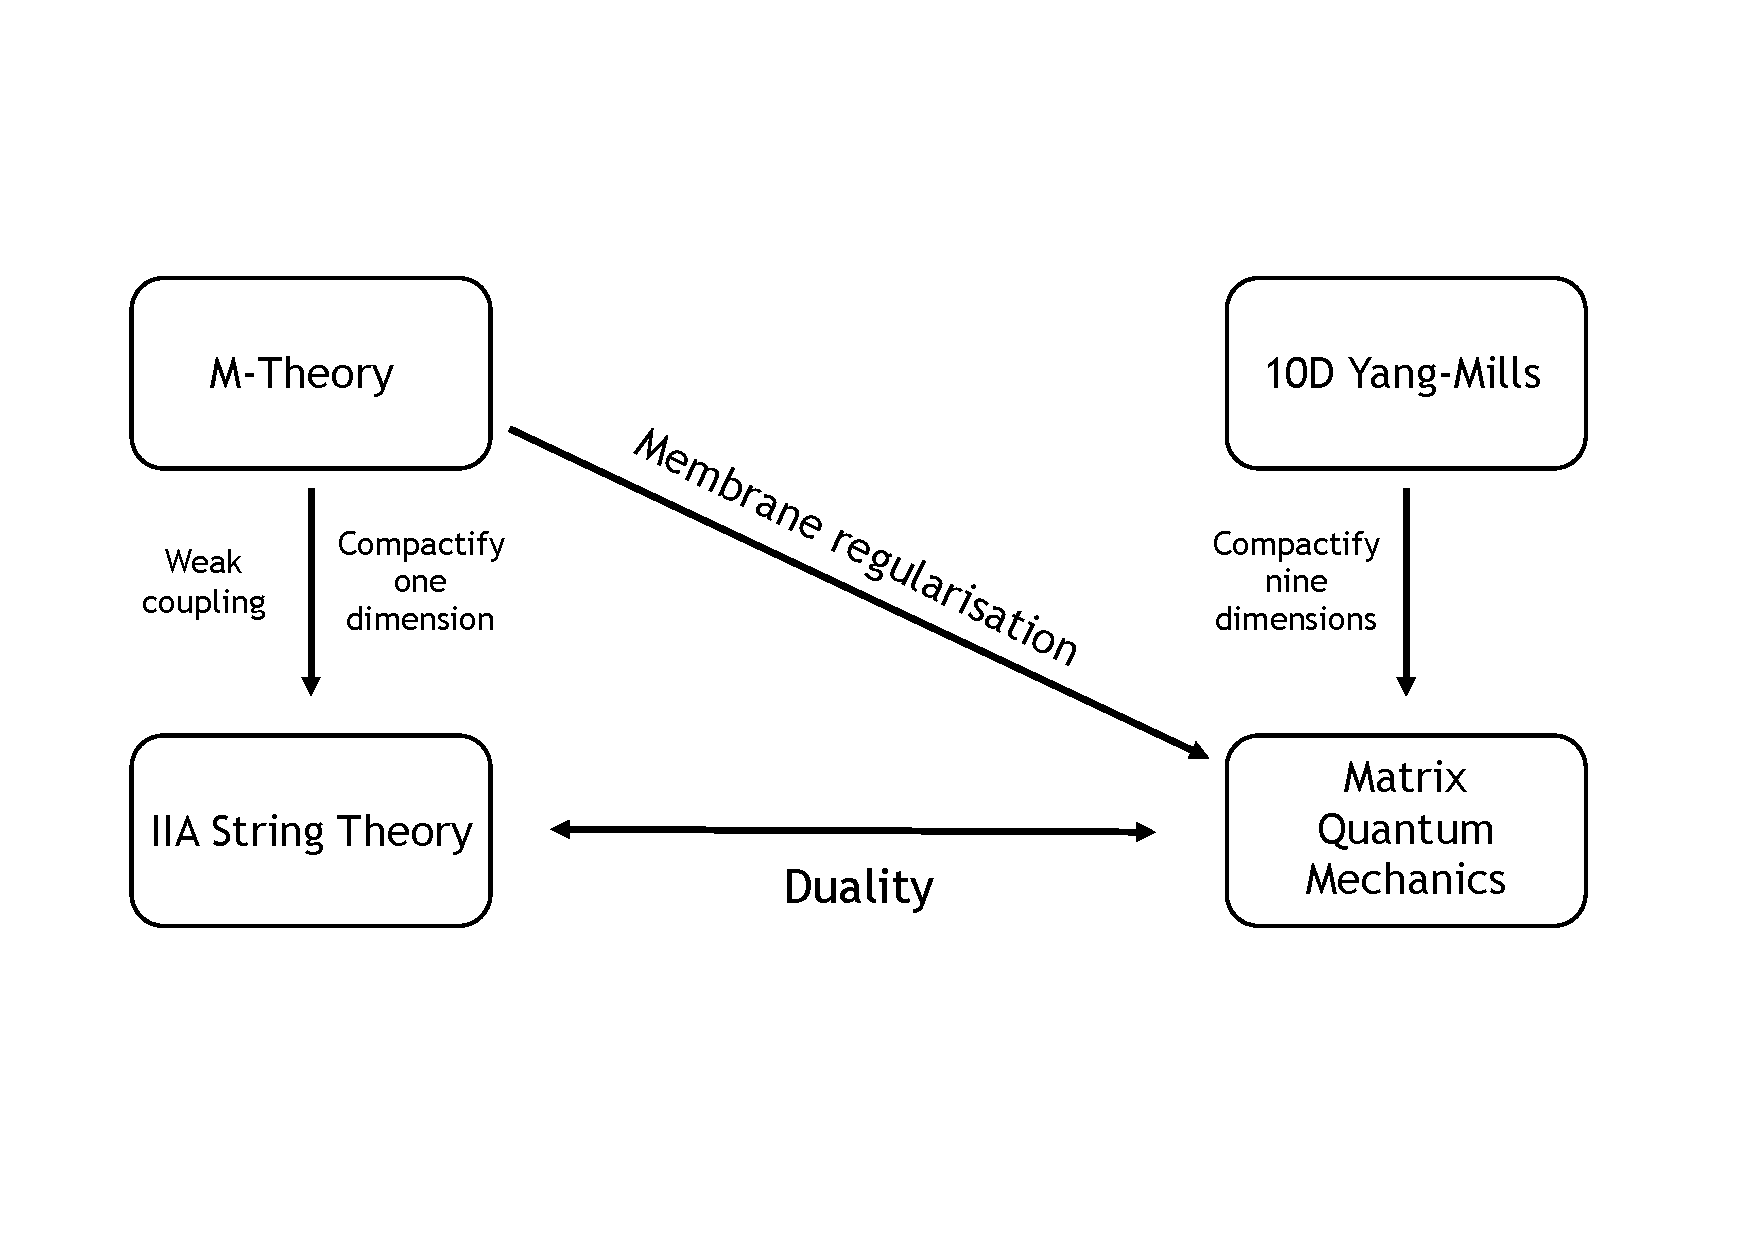
\includegraphics[scale=0.5]{duality}
\caption{The correspondence between supersymmetric matrix quantum mechanics and M-theory. In this limit the type IIA string theory is in a specific frame, the infinite momentum frame ($N\to\infty$).}
\label{duality}
\end{figure}   

The original proposal \cite{Berenstein2002} for general flux $\mu$ was supposed to give a description of the Discrete Light Cone Quantization (DLCQ) of M-theory on the maximally supersymmetric pp-wave background\footnote{For general plane-wave backgrounds see \cite{Blau2004}.} of eleven dimensional supergravity
\be \label{ppwave}
ds^2=-2dx^+dx^-+\sum_{A=1}^9dx^Adx^A-\left(\sum_{i=1}^3\frac{\mu^2}{9}x^ix^i+\sum_{a=4}^9\frac{\mu^2}{36}x^ax^a\right)dx^+dx^+,
\ee
with 
\begin{align}
F_{123+}=\mu~~~~~,~~~~~
x^{\pm}=\frac{t\pm x}{\sqrt{2}}. 
\end{align}
In the large N limit with fixed momentum $p=\frac{N}{R}$ and fixed $\mu$, this matrix quantum mechanics model should describe M-theory on the pp-wave \eqref{ppwave} background  in a sector with boost-invariant momentum parameter $\mu p$. 

We can write the bosonic part of the potential of \eqref{HamiltonianBMN} in sum of positive terms such as 
\be \label{BMNpotential}
V=\frac{R}{2}\Tr{\left[\left(\frac{\mu}{3R}X^i+i\epsilon_{ijk}X^jX^k\right)^2+\left(\frac{\mu}{6R}\right)^2X_aX^a\right]}.
\ee 
Then the types of vacua of this theory are manifest. They are 
\begin{itemize}
	\item $X^a=0=X^i~,~i=1,2,3~,a=4,\cdots, 6$ and corresponds to the trivial vacuum
	\item $X^a=0~,a=4,\cdots,9$ and $X^i=\frac{\mu}{3R}J^i~,i=1,2,3$, with $J^i$ being the generators of $SU(2)$ and corresponds to the non-trivial vacuum. 
\end{itemize} 

Among the quantum mechanics data and the gravity data there is only one relationship  
\be 
\text{matrix elements} ~X~~ \longleftrightarrow ~~\text{D0-branes},
\ee 
and this is sufficient to reconstruct all the contents of gravity. The last statement has to do with the remarkable properties of D0-branes, which in presence of suitable fluxes they can polarize into D2- and NS5-branes. Then studying only $X$ amounts to study all the contents of the gravity theory in the following way.  Each diagonal element of $X$ corresponds to the position of of each D0-brane in the gravity side, and the non-diagonal elements to stringy interactions among the D0's, see figure \ref{matrix}. This is understood in the following way. Being the matrices $X$ (sub)part of the Yang-Mills theory\footnote{In particular it is dimensional reduction of it as we saw.} they also transform under the adjoint representation of  $U(N)$ symmetry because of unitarity. We recall that under the same representation transforms an open string. Hence, both for the matrix and the string we need two indices to label the "state", which from the matrix point of view these indices can be realized as indices labeling the entries of the matrix, while from string perspective these are the Chan-Paton indices. Thus, for instance a string stretching from D-brane 1 to D-brane 2 is labeled as 12 and corresponds to the $x_{12}$ entry of the matrix. Similarly, strings ending on the same D-brane are denoted with same indices, but since D0-branes are point-like the information we get is that this open string actually begins and ends on the same point.   Then from this point of view it is understood that since the size of the matrix is $N\times N$ we have to take $N$ large such that we reconstruct more and more information about the gravity data.  

Furthermore, the BMN matrix model has one more scale given by the mass $\mu$. Then one can construct an effective coupling as $g_{\text{eff}}=\frac{\lambda}{\mu^3}$, where $\lambda$ is the t'Hooft coupling $\lambda=g_{YM}^2N$.  This effective coupling controls the regimes of validity of the descriptions. Weak coupling ($g_{\text{eff}}\ll1$) is when the matrix theory is valid and perturbation analysis can be applied with $g_{\text{eff}}$ as expansion parameter. Strong coupling ($g_{\text{eff}}\gg1$) is when the supergravity description is valid.  In this paper we are interested in the gravity description for the bosonic sector of the model.

\begin{figure}[h]
	\centering
	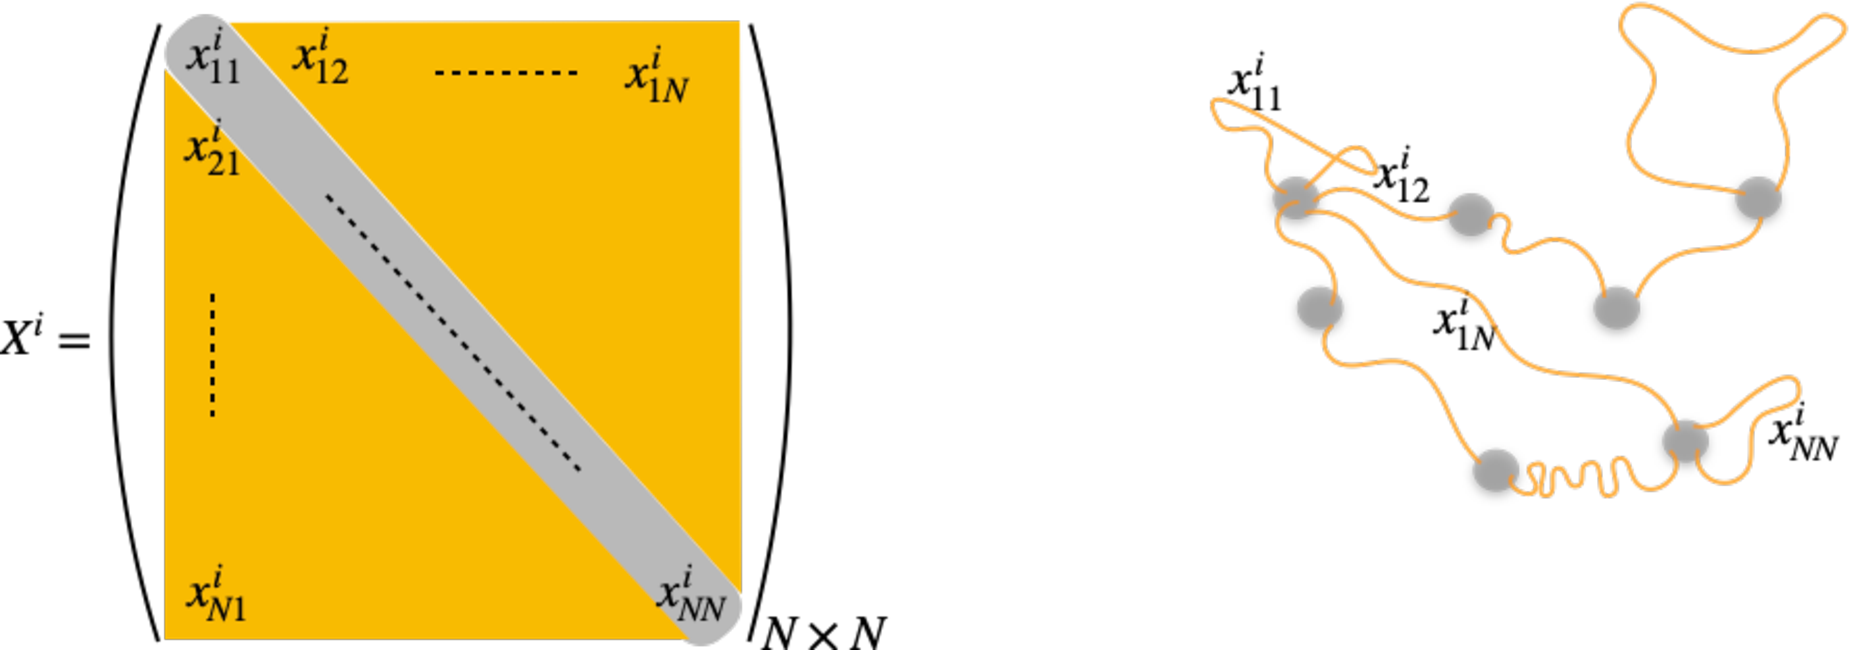
\includegraphics[scale=0.4]{matrix}
	\caption{The correspondence between the matrices of quantum mechanics and D0-branes of string theory. Diagonal elements contain information for the positions of D0's while non-diagonal elements indicate interactions between them. The D0-branes are point-like, hence an entry $x_{ii}$ gives the "location" of the i-th D0-brane.}
	\label{matrix}
\end{figure}
In addition we comment to the interpretation of the solutions of the BMN potential \eqref{BMNpotential} from the gravity point of view. The trivial vacuum corresponds to placing $N$ D0-branes in $r=0$ in the gravity side creating in this way a black hole-like object in type IIA supergravity with $SO(3)\times SO(6)$ symmetry. In the BFSS model this realizes the metric of $N$ coincident D0-branes since the $SO(8)$ symmetry naturally appears there. From M-theory point of view, this vacuum is believed to be due to a single 5-brane   \cite{Maldacena2003}. On the other hand, the number of non-trivial vacua can be organized in partitions of $N$ as $\{N_1,\cdots,N_k\}$.  Geometrically they are supposed to correspond to concentric fuzzy shells in three dimensions placed in the center of the transverse six dimensions, with each shell having  radius $r_i\sim\frac{N_i\mu}{6R}$ \cite{Berenstein2002},\cite{Dasgupta2002}. 



Nevertheless there has being a lot of progress towards understanding of the matrix models in the context of (quantum) gravity \cite{Bergner2019}, \cite{Catterall2010}, \cite{Hanada2014}, \cite{Nishimura2012}, \cite{Masanori2017}. In this paper, we have organized the contents as follows. In the next section we investigate the dynamical behavior of D0-branes in a specific background, in particular in a symmetry reduced, classical pp-wave background. We do this by firstly calculating the force that a single (probe) D0-brane feels once it has been inserted in this background and secondly by calculating the force a probe D2-brane feels in the same background. One can think that this D2-brane can be realized as consisting of a large number ($q$) of D0-branes. Furthermore, in section \ref{Vacua}  we repeat the analysis for a D0-brane in a background that geometrically corresponds to the trivial vacuum solution of the BMN both in zero and finite temperature. 


\section{Force in symmetry reduced pp-waves: a warm up}\label{classicalforce}
In this section we start by calculating the force that a D0-brane feels in a classical plane wave background in ten dimensions and then repeating the calculation for a D2-brane. The starting point is  an eleven dimensional metric which is a symmetry reduced version of the \eqref{ppwave}
\be \label{unboosted}
ds^2=-(1+\frac{Q^2}{4})dt^2+(1-\frac{Q^2}{4})(dx^{10})^2-\frac{Q^2}{2}dtdx^{10}+\sum_{i=1}^{3}dx_idx_i+\sum_{a=4}^9dx_adx_a,
\ee 
where Q is defined as \footnote{This $\mu$ is the deformation parameter, and it is the same that appears in the matrix model \eqref{HamiltonianBMN}.}
\be \label{Fdefin}
Q^2\equiv\frac{\mu^2}{9}\sum_{i=1}^3(X^i)^2+\frac{\mu^2}{36}\sum_{a=4}^9(X^a)^2,
\ee
 and the 4-form field is given as 
\be 
Q_{123(10)}=-Q_{0123}=\frac{\mu }{2}.
\ee
We note that this metric, is written in the unboosted frame. Since any pp-wave metric is boost covariant \cite{Blau2004}, the effect of boosting is simply to rescale the deformation parameter $\mu$.  We furthermore note that this background is a general background that should capture general (but symmetry reduced) features of the BMN matrix model and in fact one can derive the action of the BMN from this metric \cite{Dasgupta2002}, \cite{TaylorIV1999}.

\subsection{A D0-brane feels only the trivial vacua}
We want to perform a compactification of \eqref{unboosted} along the  spacelike $x^{10}$ direction to make contact with the ten-dimensional theory. One easy way to obtain this is to write down the relation between the 11D-metric and the 10D-metric
\be 
ds^2_{11}=e^{-\frac{2\phi}{3}}ds_{10}^2+e^{\frac{4\phi}{3}}\left(dx^{10}-C_\mu dx^\mu\right)^2.
\ee

\noindent
Then, the ten-dimensional metric is given as 
\be \label{compacified}
ds^2_{10}=-\left(1-\frac{Q^2}{4}\right)^{-\frac{1}{2}}dt^2+\delta_{ab}\left(1-\frac{Q^2}{4}\right)^{\frac{1}{2}}dx^adx^b,
\ee
with 
\be 
e^{\frac{4\phi}{3}}=1-\frac{Q^2}{4},~~C_0=-\frac{Q^2}{4-Q^2}dt,~~ Q_{0123}=-\frac{\mu }{2},~~ H_{123}=\frac{\mu}{2}.
\ee
Here $C_0$ is the RR-one form potential, $H_{123}$ is the NS-NS three-form potential and $F_{0123}$ is the RR three-form field strength. These form fields arise from the distribution of the eleven-dimensional three form into the R-R and NS-NS sector.  Geometrically, this corresponds to distributing the eleven dimensional momentum into different geometric configurations, like the D-branes.

By direct calculation of the Ricci scalar of \eqref{compacified}, we find 
\begin{align} \nn
\mathcal{R}=\frac{\mu ^2}{5184}\left(1-\frac{Q^2}{4}\right)^{-\frac{5}{2}}\sum_{i=1}^3\sum_{a=4}^9 \Bigg\{&\mu ^2(7-Q^2) \Big[(X^a)^4+48 (X^a)^2 (X^i+3)+96 X^a (X^i)^2\\
\nn&+16 (X^i)^2 \left((X^i)^2+36\right)\Big]\\ 
&+252 \left[(X^a)^2+4 \left((X^i)^2+9\right)\right] Q-63 \left[(X^a)^2+4 \left((X^i)^2+9\right)\right] Q^3 \Bigg\}
\end{align}
From this we see that we can trust the supergravity solution \eqref{compacified} only in the low curvature region, i.e when $\frac{Q^2}{4}\ll 1$. 

\noindent
In this limit one can expand as follows 
\begin{align}\nn
 e^{-\frac{2\phi}{3}}&\approx 1+\frac{Q^2}{8}+\mathcal{O}\left(Q^4\right)\\
 \nn C_0&\approx-\frac{Q^2}{4} +\mathcal{O}\left(Q^4\right).
\end{align}

Having set up the playground, now we turn to calculate the force. When we do this, we have in mind a situation when we naively place a D-brane probe in the spacetime and ask for its dynamical behaviour. To this end, we need to write down the DBI action for the D0-brane by choosing the gauge where the parameter of the worldline of the D0 coincides with the time component of the spacetime. In a general background, it is given by 
\be\label{bosonicpart}
S_{D_0}=-T_0\int dt e^{-\phi}\sqrt{-g_{\mu\nu}\frac{dx^\mu }{dt}\frac{dx^\nu}{dt}}+T_0\int dt C_0,
\ee
where $T_0=\frac{M_s}{g_s}$ is the tension of the D0-brane and the expression inside the square root is the pull-back of the spacetime metric on the worldline of the D0-brane. We remind that a Dp-brane naturally couples with a p+1 form, thus the only form that couples to a single D0-brane is the one-form potential $C_0$.  Then, the action reads as 
\be 
S_{D_0}=-T_0\int dt \left(1+\frac{3Q^2}{16}\right)\sqrt{1+\frac{Q^2}{8}-\left(1-\frac{Q^2}{8}\right)\dot{x}^2}+T_0\int dt \left(-\frac{Q^2}{4}\right).
\ee
Moreover, after taking the non-relativistic limit we expand the action up $\dot{x}^2$ and $Q^2$ terms leading to
\be 
S_{D_0}\approx-T_0\int dt\left[1+\frac{Q^2}{2}-\frac{1}{2}\dot{x}^2\right] +\mathcal{O}(Q^4,\dot{x}^4).
\ee
One can read off the potential from this action:
\be \label{potential1}
V_{D_0}(x)=T_0(1+\frac{Q^2}{2}).
\ee
Recalling \eqref{Fdefin} we write the potential as, 
\be 
V_{D_0}(X^i,X^a)=T_0\left[1+\frac{1}{2}\left(\frac{\mu^2}{9}\sum_{i=1}^3(X^i)^2+\frac{\mu^2}{36}\sum_{a=4}^9(X^a)^2\right)\right].
\ee

\noindent
We see an explicit dependence of $\mu$ in the potential. It is also worth noting that the trivial vacua ($X^i=0$ and $X^a=0$) are supersymmetric solutions of the potential after performing a shift, but the non-trivial $SU(2)$ vacua are not. The latter, geometrically are believed to correspond to concentric fuzzy spheres, however the single D0-brane in this background is agnostic if there are any fuzzy spheres at all. Had we consider a different probe, for example a D2-brane, then this would couple to higher forms and would give rise to the $SU(2)$ part of the potential. This is demonstrated in the next subsection. 

\noindent
Furthermore, we regard the terms inside the sum as the radii of an $S^2$ and $S^5$ sphere. In other words we can write the potential as  
\be 
V_{D_0}(r_2,r_5)=T_0\left[1+\frac{1}{2}\left(\frac{\mu^2}{9}r_2^2+\frac{\mu^2}{36}r_5^2\right)\right],
\ee
where $r_2$ denotes the radius of the $S^2$ sphere and $r_5$ the one of $S^5$. In addition we can restrict the D0-brane to move only in some of the directions of the spacetime, for example we can place it in the trivial vacua  $X^a=0$ corresponding to $r_5=0$ and then it would feel only the presence of the $S^2$ sphere. However, this is a naive picture because the hole system is studied at the classical level. According to matrix model simulations, the matrices are never zero but they subject to quantum fluctuations independent of which vacuum one studies \cite{Bergner2019}, \cite{Catterall2010}, \cite{Hanada2014}, \cite{Masanori2017}.  

\noindent
From this potential one can obtain the force that the D0-brane feels by differentiating with respect to the radial coordinate. This is simply given by 
\be 
F_{D_0}(r_2,r_5)=-T_0\frac{\mu^2}{9}\left(r_2+\frac{r_5}{4}\right).
\ee  



\subsection{A D2-brane feels the $SU(2)$ vacua}
In this section we calculate the force that a D2-brane probe feels in the weakly curved background \eqref{compacified}. One can think this D2 probe as being made of ($q$) D0-branes where the number of D0's is taken to be large. However, in order to consider this as a probe, one has to require that the probe charge $q$ is much less than the background charge $N$, i.e we are studying the limit $1\ll q\ll N$. We can imagine this brane to have a $S^2$ topology embedded in a three dimensional space. In particular, one natural embedding would be along the $SO(3)$ part of the metric where the other six dimensions are transverse to it. For convenience, we place the D2-brane in the center of the the six transverse directions such that $X^a=0$. Then the DBI and WZ action of the D2-brane will be of the familiar form 
\be \label{D2action}
S_{D_2}=-T_2\int d^3\sigma e^{-\phi}\sqrt{-\det\left(G_{ab}+2\pi\alpha'\mathcal{F}_{ab}\right)}+T_2\int\left(C_3+2\pi\alpha'\mathcal{F}_2\wedge C_1\right),~~~q\ll N
\ee    
where $2\pi\alpha'\mathcal{F}_2=2\pi\alpha'F_2-B_2$. As in the case of the D0-brane, one can also choose the static gauge here, which corresponds to identifying the worldvolume dimensions with the three dimensional part of the sub space of the ten-dimensional spacetime. We can choose $t,\theta, \phi$ coordinates parametrizing the $S^2$. The radius of $S^2$ is given by $r$, while the angles have the usual ranges $\theta\in [0,\pi]$, $\phi\in[0,2\pi]$. For a compact D2-brane of arbitrary topology the total  charge $q$ is quantized and it is given as  
\be 
\int_{S^2}F_2=2\pi q ~~~\longrightarrow~~~ F_2=\frac{1}{2}q\sin\theta d\theta\wedge d\phi.
\ee 
We note that the integer $q$ is also related to the first Chern class of the U(1) bundle at a fixed point in time and moreover, it acts as a source for the R-R vector field and the interpretation of it is the number of D0-branes that are bound on the surface of the D2-brane. 

\noindent
Analogously, the forms are given in the static gauge as 
\begin{align} 
C_1&=\left(1-\frac{Q^2}{4}\right)^{-1}dt\\
C_3&=\frac{1}{3}\mu dt\wedge S_2~~~,~~~S_2=\frac{1}{2}\epsilon_{ijk}x^i\wedge dx^j\wedge dx^k,~~i,j,k=1,2,3.
\end{align}
Furthermore, the pullbacks of the metric $G_{ab}$ on the D2-brane are given as 
\begin{align}
\det{g_{tt}}&=-\left(1-\frac{Q^2}{4}\right)^{-\frac{1}{2}}\\
\det{g_{\perp}}=\det({g_{\theta\theta}g_{\phi\phi}})&=\left(1-\frac{Q^2}{4}\right)r^4\sin^2\theta.
\end{align}
\noindent
From these we have that 
\begin{align}
F_{\theta\phi}&=\frac{1}{2}q\sin\theta\\
F_{ab}F^{ab}&=\frac{q^2}{2\left(1-\frac{Q^2}{4}\right)r^4}\\
\det{F_2}&=\frac{1}{2}F_{ab}F^{ab}\det{g_{\perp}}=\frac{q^2}{4}\sin^2\theta.
\end{align} 

%The action can be written as (ignoring the part coming from the $B_2$ field for the moment) 
%\be 
%S=-T_2\int dtd\theta d\phi\left[\pi\alpha'q\sin\theta\left(1-\frac{F^2}{4}\right)^{-\frac{1}{4}}+\left(1-\frac{F^2}{4}\right)^{\frac{3}{4}}\frac{r^2\sin\theta}{2\pi\alpha'}-\textcolor{red}{\frac{4\pi\mu r^3}{3}}+\pi\alpha'\left(1-\frac{F^2}{4}\right)^{-1}q\sin\theta\right].
%\ee
%\be 
%S=-T_2\int dtd\theta d\phi \left[\left(1-\frac{F^2}{4}\right)^{-1}\pi\alpha' q\sin\theta+\frac{r^4\sin\theta}{2\pi\alpha' q}-\frac{r^3\mu }{6}-\left(1-\frac{F^2}{4}\right)^{-1}\pi\alpha' q\sin\theta\right].
%\ee
\noindent
The DBI action can be written as
\be 
S_{DBI}=-T_2\int d^3\sigma e^{-\phi}\sqrt{-\det{g_{tt}}}\left(\det{g_{\perp}+2\pi\alpha'\det{F_2}}\right)^\frac{1}{2},
\ee 
and considering the main contribution coming from $\det{F_2}$\footnote{This amounts to $\frac{q^2}{4}\sin^2\theta\gg 1$, reflecting the fact that the charge $q$ is large but nevertheless we are in the limit $q\ll N$ }, we can expand the action around this and get
\be 
S_{DBI}\approx-T_2\int d^3\sigma e^{-\phi}\sqrt{-\det{g_{tt}}}\left(2\pi\alpha'\sqrt{\det{F_2}}+\frac{\det{g_{\perp}}}{4\pi \alpha'\sqrt{\det{F_2}}}\right).
\ee 
Using the exact expressions this gives 
\begin{align}\nn
S_{DBI}&\approx-T_2\int dt d\theta d\phi\left[\left(1-\frac{Q^2}{4}\right)^{-1}\pi\alpha' q\sin\theta+\frac{r^4\sin\theta}{2\pi\alpha' q}\right]\\
&\approx -T_2\int dt\left[\left(1-\frac{Q^2}{4}\right)^{-1}4\pi^2\alpha' q+\frac{2r^4}{\alpha' q}\right].
\end{align}
Similarly the WZ action gives 
\be 
S_{WZ}=T_2\int dt \left[\frac{4\pi\mu r^3}{3}+4\pi^2\alpha' q\left(1-\frac{Q^2}{4}\right)^{-1}\right].
\ee

We see that the leading terms cancel each other, the subleading terms that remain can be mapped to the  commutator term $\sim\Tr [X^i,X^j]^2$ and the Myers term $\sim-\Tr\left(i\frac{\mu }{3}\epsilon_{ijk}X^iX^jX^k\right)$ in the BMN model. In addition, one could also be interested in the contributions coming from the $B_2$ field. However, as it is shown in \cite{Taylor2000b} the contributions of $B_2$ coming from WZ and DBI action cancel each other. Nevertheless, we can add a term $\sim \mu^2 r^2$ such that we complete the square in the action. This will make the interpretation more clear. By adding and substracting this term,  the action is given as  
\be 
S_{D_2}\approx-\frac{2T_2}{\alpha' q}\int dt\left[\left(r^2-\frac{2\pi\mu\alpha' q}{3}r\right)^2-\frac{4\pi^2\mu^2\alpha'^2q^2r^2}{9}\right].
\ee
The potential is simply 
\be 
V_{D_2}(r)=\frac{2T_2}{\alpha' q}\left[\left(r^2-\frac{2\pi\mu\alpha' q}{3}r\right)^2-\frac{4\pi^2\mu^2\alpha'^2q^2r^2}{9}\right].
\ee
From this we see that apart from the trivial $r=0$ solution, there is a non-trivial equilibrium radius at 
\be 
r=\frac{4\pi\alpha'q\mu}{3}.
\ee 
This is understood as the radius in which the contraction that is caused by the $r^2$ and $r^4$ terms compensates with the expansion caused by the $r^3$ term in the potential. In fact one can generalize this and have a number ($k$) of concentric D2-branes instead of just one. Then for each D2-brane there is an equilibrium radius given by 
\be 
r_i=\frac{4\pi\alpha'q_i\mu}{3},
\ee   
with $q_i$ being the charge of the i-th D2-brane. In the Matrix model side instead, this picture corresponds to a particular copy of the $N$ dimensional representation of $SU(2)$ up to a non-commutative factor in the case of a single D2-brane and a partition $\{N1,\cdots,N_k\}$ of the $N$ dimensional representation of $SU(2)$ in the case of $k$ concentric D2-branes .  

The force that the D2 feels from the background is given as 
\be 
F_{D_2}(r)=-\frac{8T_2}{\alpha' q}r^2(r-\pi q\alpha'\mu).
\ee
In fact, we see that it is independent of the configuration of the geometry, for example independent of the warp factor $e^\frac{2\phi}{3}$, but it does depend on its own charge $q$ and the flux parameter $\mu$, in accordance with the D0-brane case. We also see that the force becomes repulsive for $r\in (0,\pi q\alpha'\mu)$. This results to an interpolation from a strong, attractive force to a soft repulsive force after going through the minimum of the potential.  In the minimum, we have a D2-brane freely sitting on a position in spacetime. So in this way, we can use them as  probes to the geometry. 


\section{BMN vacua}\label{Vacua}
In this section, after discussing the matrix model vacua and how one can think this as a electrostatic configuration problem following \cite{Lin2006}, we describe the gravity duals and we compute the force of the D0-brane for the trivial vacuum of the BMN.  For similar discussions see \cite{Lozano2017}, \cite{Lin2004a}, \cite{Costa2015}.
\subsection{Generic analysis}
In general, we should look for a gravity solution that preserves half of the supersymmetries\footnote{This is because the BMN model has various BPS states, but here in particular we are interested for 1/2-BPS states.} and respects the $SO(3)\times SO(6)$ symmetry. This can be motivated from the specific form of the Hamiltonian of the matrix model \eqref{HamiltonianBMN} since the gravity solution should respect the symmetries therein.  The most general solution in type IIA string theory that meets these conditions is \cite{Lin2006}
\be \label{IIAmetric}
ds^2_{10}=\left(\frac{\ddot{V}-2\dot{V}}{-V''}\right)^\frac{1}{2}\left[-\frac{4\ddot{V}}{\ddot{V}-2\dot{V}}dt^2-\frac{2V''}{\dot{V}}\left(d\rho^2+dz^2\right)+4d\Omega_5^2+2\frac{V''\dot{V}}{\Delta}d\Omega_2^2\right],
\ee 
with
\begin{align*}
\dot{V}&=\rho\p_{\rho} V~,~\ddot{V}=\rho\p_{\rho}(\dot{V}),~
~V'=\p_{z}V~,~V''=\p^2_zV,\\
\Delta&=\left(\ddot{V}-2\dot{V}\right)V''-\left(\dot{V}'\right)^2,
\end{align*}
and the dilaton and NS-NS and R-R forms are given as 
\begin{eqnarray}
&e^{4\phi}=\frac{4(2\dot{V}-\ddot{V})^3}{V''\dot{V}^2\Delta^2},~~&B_{2}=2\left(\frac{\dot{V}\dot{V}'}{\Delta}+\rho\right)d\Omega_2\nonumber\\
&A_1=\frac{2\dot{V}\dot{V}'}{2\dot{V}-\ddot{V}}dt,~~&A_3=-\frac{4\dot{V}^2V''}{\Delta}dt\wedge d\Omega_2.
\end{eqnarray}
In \eqref{IIAmetric} appears a function $V(z,\rho)$. In fact this function can be interpreted as a potential that sources different brane (NS5, D2, D0) configurations, and depending on the specific form of this function one realizes different gravity solutions, which correspond to different vacua in the matrix model side.  We are interested in the bosonic sector of BMN because in that case we can write a metric ansatz that respects the bosonic symmetries. In the BMN case, we see from \eqref{HamiltonianBMN} that these symmetries are $R\times SO(3)\times SO(6)$. The first of these implies that there is a Killing vector associated to translations of the time coordinate. The second, implies that we can imagine a sector of the spacetime to consist of a $S^2$ sphere while the third the existence of a $S^5$ sphere, on which the bosonic generators act. Thus one can analyze solutions in eleven dimensions by using only three variables, say $x_1,x_2,y$ which satisfy the Toda equation in three dimensions \cite{Lin2004},\cite{Lin2006}
\be \label{toda}
\left(\p_{x_1}^2+\p_{x_2}^2\right)V+\p_y^2V=0.
\ee
In fact, it turns out that $y=r_2r_5^2$, where $r_2,r_5$ are the radii of the $S^2$ and $S^5$ respectively. Exploiting the translational invariance under one coordinate ($x_1$), and after changing variables $(x_2,y)\mapsto(\rho,z)$ one can recast this equation to the Laplace equation in a three dimensional space \cite{Lin2004}
\be \label{Laplace}
\frac{1}{\rho}\p_\rho\left(\rho\p_\rho V\right)+\p_z^2V=0.
\ee
We note that this three-dimensional space is not a sub-part of the ten dimensional one but rather maps to an electrostatic problem in a three dimensional space, where all gravity solutions are classified by $\rho,z$. Here, both $\rho$ and $z$ are radial (scale) coordinates, the former captures  the size of fivebranes and the latter the positions of the conducting disks, which is actually being set by the five-branes.  
If one, naively tries to find a gravity solution by just plugging in a solution of  \eqref{Laplace} into the metric \eqref{IIAmetric} will end up with singular gravity solutions. To avoid this, one has to impose boundary conditions at $y=0$ such that $V(y=0)=0$. This condition corresponds to regimes with vanishing radii of $S^2$ or $S^5$. Indeed $S^2$ shrinks for constant $z$ in the $z,\rho$ space (see figure \ref{rzplane}) and $S^5$ shrinks between two nearby disks in the $\rho=0$ line. 


In the case of the BMN model, the asymptotic expansion is decomposed in two parts of which the first one represents the electrostatic potential and the second one the specific electrostatic configuration imposed by the boundary conditions. We note that this means that one can specify the solution but not necessary to which vacuum corresponds, since there will be vacua with the same boundary conditions. The first non-trivial potential is \cite{Maldacena2003}
\be \label{dipole}
V\approx \rho^2 z-\frac{2}{3}z^3+\mathcal{P}\frac{z}{\left(\rho^2+z^2\right)^\frac{3}{2}},
\ee
where $\mathcal{P}$ is a short of dipole sub-leading correction, produced by the conducting disks and their images with respect to the infinite conducting plane at $z=0$. Its value is given by 
\be 
\mathcal{P}=2\sum_iz_i\mathcal{Q}_i\sim N,
\ee
where $i$ runs over the various disks, $\mathcal{Q}_i$ is the charge of the $i$-th disk and $N$ is the number of D0-branes.\footnote{Here we make contact with the introductory remarks, where we stated that all the contents can be reconstructed from D0-branes.} The number of D0-branes can be extracted from the particular configurations of the disks. Suppose for example that there is a finite set of conducting disks at positions $z_i=\frac{\pi}{2}N_5^{i}$, with radii $R_i$ and charge $\mathcal{Q}_i=\frac{\pi^2}{8}N_2^{i}$. Then the disks are sourced by the NS5-branes in the background, with the charge $\mathcal{Q}_i$ being associated to the D2-brane charges. In this sense, one can write the number of D0-branes as 
\be 
N=\sum_{i}\left(\sum_{j<i}N_5^{j}\right)N_2^{i}.
\ee    
Furthermore, this $N_2^{i}$ is related to the copies of dimension $N_5^{i}=(2j+1)$ irreducible representations, giving a geometric realization of the situation of the matrix model.

\noindent
Plugging in \eqref{dipole} into the metric \eqref{IIAmetric} and expanding at large $\rho$ and $z$, the metric takes the form 
\be \label{largezrho}
ds^2\approx -\frac{8z^{\frac{7}{2}}}{\sqrt{15\mathcal{P}}}dt^2+2\sqrt{15\mathcal{P}}z^{-\frac{7}{2}}\left(dz^2+z^2d\Omega_2^2+d\rho^2+\rho^2d\Omega_5^2\right)+\cdots,
\ee
where we have keep only the leading terms on $z$ and $\rho$ and the relevant piece of metric that still has the $SO(3)\times SO(6)$ symmetry. The dots above denote mixing and subleading terms. We note that the part inside the parenthesis is actually $\mathbb{R}^9$, which is written in a way that makes the symmetries of the theory manifest. One can further change coordinates 
\be \label{coordchange}
r^2=16\left(\rho^2+z^2\right),
\ee
 and in the large $r\to \infty$ limit the metric  \eqref{largezrho} approximates the near horizon geometry of $N$ coincident D0-branes
\be \label{larger}
ds^2\approx -H(r)^{-\frac{1}{2}}dt^2+H(r)^{\frac{1}{2}}\left(dr^2+r^2d\Omega_8^2\right)+\cdots,~~~H(r)\approx \frac{256\cdot 15\mathcal{P}}{r^7}.
\ee
 

\subsection{Trivial vacuum}
From the gauge theory side, it seems that the easiest classical vacuum, is the one that all matrices vanish trivially, i.e $X^i=0=X^a$, with $ i=1,2,3~~,~~a=4,\cdots,9$. This corresponds to the situation where we have  $N$ copies of the trivial ($j=0$) representation of $SU(2)$, and in the electrostatic description this translates to a single disk at a distance close to (of order one unit) the infinite conducting disk at $z=0$ (see figure \ref{rzplane}). In the gravity side the picture is the following: $N$ corresponds also to the number of D0-branes  and putting these in the $r=0$ position of the spacetime creates a singular geometry  \eqref{larger}. However, the situation in BMN model is a bit different, because one has to realize also the correct symmetries, namely $SO(3)\times SO(6)$. This vacuum is believed to correspond to a single fivebrane in the gravity side \cite{Maldacena2003}, but the gravitational approximation is not very good near the fivebrane  \cite{Berenstein2002}, \cite{Lin2006}. Nevertheless, one might hope to perform an expansion in the metric in the large $\rho$ limit while keeping $z$ of order one. This translates to 
\be 
r^2=16\left(\rho^2+z^2\right)\gg1,~~\rho\gg1,~~~z\sim\mathcal{O}(1).
\ee 
\subsubsection{Zero temperature}
We will start applying this to zero temperature first and then move to finite T in the next subsection. After taking the large $r$ and then the trivial vacuum limit, we get a metric of the form 
\begin{align} \label{trivialvac}
ds^2&= -H(r)^{-\frac{1}{2}}dt^2+16H(r)^{\frac{1}{2}}\left(dz^2+z^2d\Omega_2^2\right)+H(r)^{\frac{1}{2}}\left(dr^2+r^2d\Omega_5^2\right),\\ H(r)&\equiv \frac{256\cdot 15\mathcal{P}}{r^7},\\
e^\phi&=\left(\frac{2^{12}15\mathcal{P}}{r^7}\right)^\frac{3}{4},%-\frac{21}{\sqrt{2}}\left(\frac{\left(15^3\mathcal{P}^34^{21}\right)}{r^{29}}\right)^\frac{1}{4} \text{leading order only}, 
\\
\label{oneform}A_1(r)&=-\frac{r^7}{2^{11}15\mathcal{P}}-\frac{7\pi^2 r^5}{4^515\mathcal{P}}-\frac{7\pi^4r^3}{4^348\mathcal{P}}+\frac{r^2}{10}-\frac{7\pi^6r}{4\cdot 384\mathcal{P}}-\frac{3\pi^2}{5},
\end{align}
\noindent
We have kept only leading orders both in the expression of dilaton and the one form. The next correction to the dilaton is of order $\mathcal{O}(r^{-29/4})$ and in the large $r$ limit we neglect it. In the same limit, the contribution of the R-R one form is significant. Furthermore, we see that in this limit and for same energy scale (or the same radius $r$), the effective curvature of the five-sphere, which in string units is the inverse of $\frac{\mathcal{R}_5^2}{\alpha'}=H(r)^{\frac{1}{2}}r^2$, is much smaller than the one of the two-sphere, which is the inverse of $\frac{\mathcal{R}_2^2}{\alpha'}=H(r)^{\frac{1}{2}}z^2$ . This means that curvature corrections coming from the two-sphere part of the metric may become important when compared with the one of the five-sphere. In fact to make the metric physically viable we should take the limit $z\sim \lambda^{1/3}$ \cite{Lin2006}\footnote{Both $r$ and $z$ here are energy scales, and this condition reflects the fact that we push the regime of validity of the metric to its boundary. In \cite{Maldacena2018}, and based on \cite{Polchinski1999} was argued that the breaking of Einstein supergravity starts at scales $\lambda^{1/3}$.}. This amounts to blow up the $S^2$ part.  We also note that the validity of the supergravity solution is when the dilaton is not too large and when the effective curvature of the five-sphere is not too big. Recalling $\mathcal{P}\sim N$ this translates to the range
\be \label{validsugra}
N^\frac{1}{7}\ll r\ll N^\frac{1}{3}.
\ee
 
\noindent
The Ricci scalar of \eqref{trivialvac}, can be computed and it is given by 
\be 
\mathcal{R}=-\frac{49\sqrt{\frac{3}{5}}}{64}\left(\frac{r^3}{\mathcal{P}}\right)^{\frac{1}{2}}.
\ee 
We see that in the regime where the supergravity description for the trivial vacuum is a good approximation, the spacetime is almost flat provided that $N$ is large.  

%Another way to see this is the following: as we pointed out, the metric \eqref{trivialvac} consists of two spheres ($S^2, S^5$), and hence two effective curvatures that control (loosely speaking) when the quantum corrections might become important. However, one should compare these with the one of the eight-sphere of the BFSS model, in the sense that the near horizon geometry of D0-branes dictates when the supergravity regime is valid. Indeed, it turns out that as long as\footnote{This is the case for finite temperature, but we comment more on this situation in section \ref{sectionfiniteT}.  } \cite{Catterall2010}, \cite{Maldacena2018}, \cite{Itzhaki1998}
%\be 
%\frac{\lambda}{U^3},~~ \text{and} ~~N,~~\text{with}~~~U\equiv\frac{r}{\alpha'}, 
%\ee
%are large, the supergravity description is valid. The inverse of this is the curvature of the eight-sphere when we are looking into the near horizon limit of D0-black brane. Here $U$ is the scale of the theory and $\lambda\equiv g_{YM}^2N$ is the t' Hooft coupling.  Comparing the warp factors and remembering that $\mathcal{P}\sim N$ we find for the trivial vacuum of the BMN that 
%\begin{align}
%\frac{\mathcal{P}}{r^3}\sim \frac{\lambda}{r^3},~~&\text{and}~~ N~~ \text{large for the}~S^5~ ,\\
%\sqrt{\frac{\mathcal{P}}{r^3}}z^2\sim\sqrt{\frac{\lambda}{r^3}}z^2,~&\text{and}~~N~~\text{large for the}~S^2~.
%\end{align}  
%Indeed we see that these conditions hold in the large $N$ limit.

Lastly, before moving to calculation of the force, it worths mentioning that after a coordinate rescalling and transformation, namely
\be 
z\to\frac{\zeta}{4}~~,~~R\to \frac{2}{5}\frac{r_0^{5/2}}{r^{5/2}},~~r_0^7\equiv 256\cdot 15\mathcal{P},~~t\to r_0t
\ee  
the metric becomes 
\be 
ds^2=\left(\frac{2}{5}\right)^{7/5}\frac{r_0^2}{R^{7/5}}\left[-dt^2+dR^2+\left(\frac{5}{2}\right)^2R^2d\Omega_5^2\right]+\left(\frac{2}{5}\right)^{-7/5}R^{7/5}\left(d\zeta^2+\zeta^2 d\Omega_2^2\right).
\ee 
We see that the near horizon limit of the vacuum solution is conformaly equivalent to $AdS_2\times S^5\times B^3$ if we keep $r_0$ fixed which means to keep $\mathcal{P}$ fixed. We also note that the "size" of the $AdS_2\times S^5$ part of the metric is much bigger than that of the $B_3$ part. Of course this was expected from the beginning since the trivial vacuum limit corresponds to large $r^2=16(\rho^2+z^2)$, with $\rho$ large and $z$ of order one.
\begin{figure}
\centering 
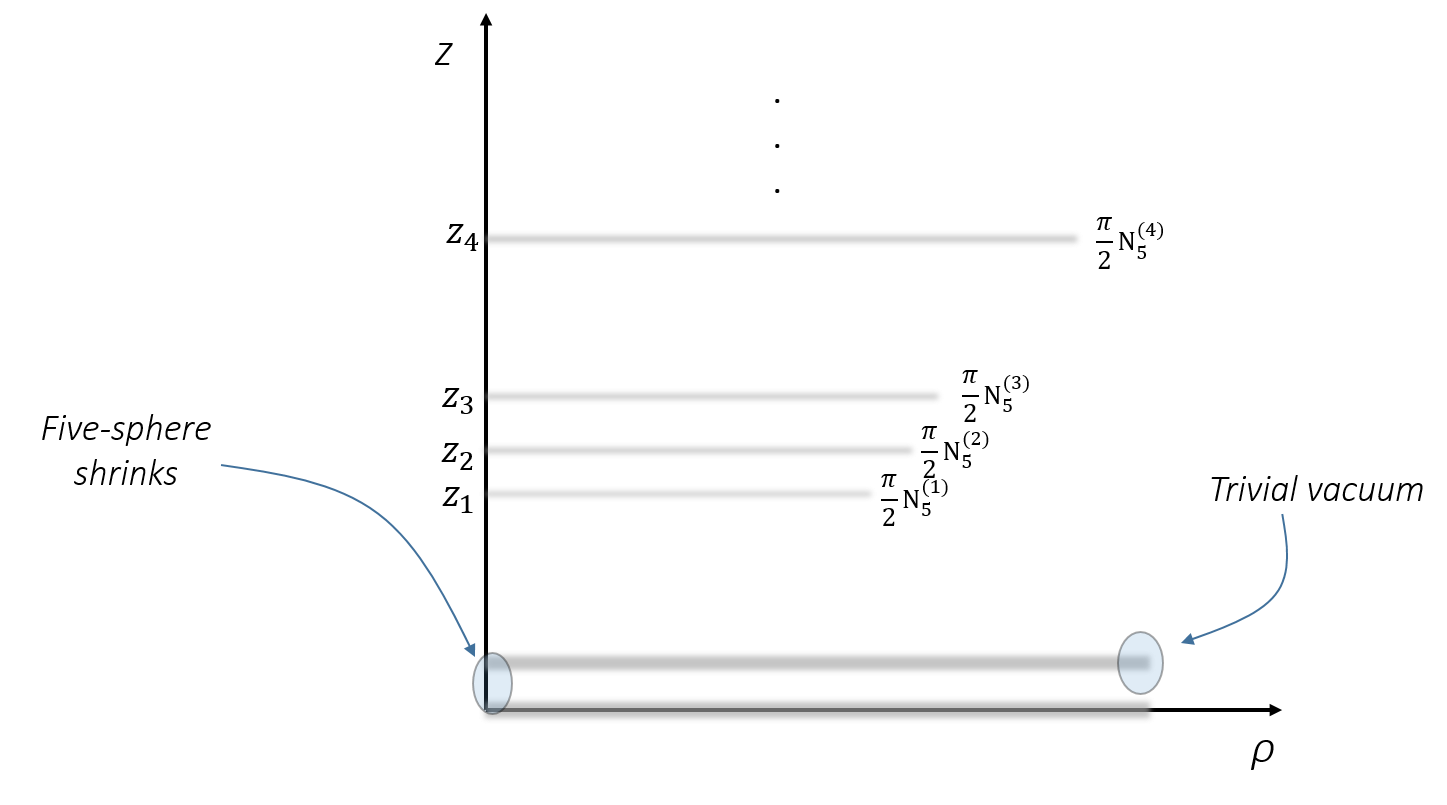
\includegraphics[scale=0.4]{zplane.png}
\caption{A cartoon of the $z-\rho$ plane. Constant $z$ lines indicate that the two-sphere shrinks while the five-sphere shrinks in the region between nearby disks near $\rho=0$. We have a conducting disk at $z=0$ which extends to infinity in the $\rho$ direction.}
\label{rzplane}
\end{figure}

\begin{figure}[h]
\centering
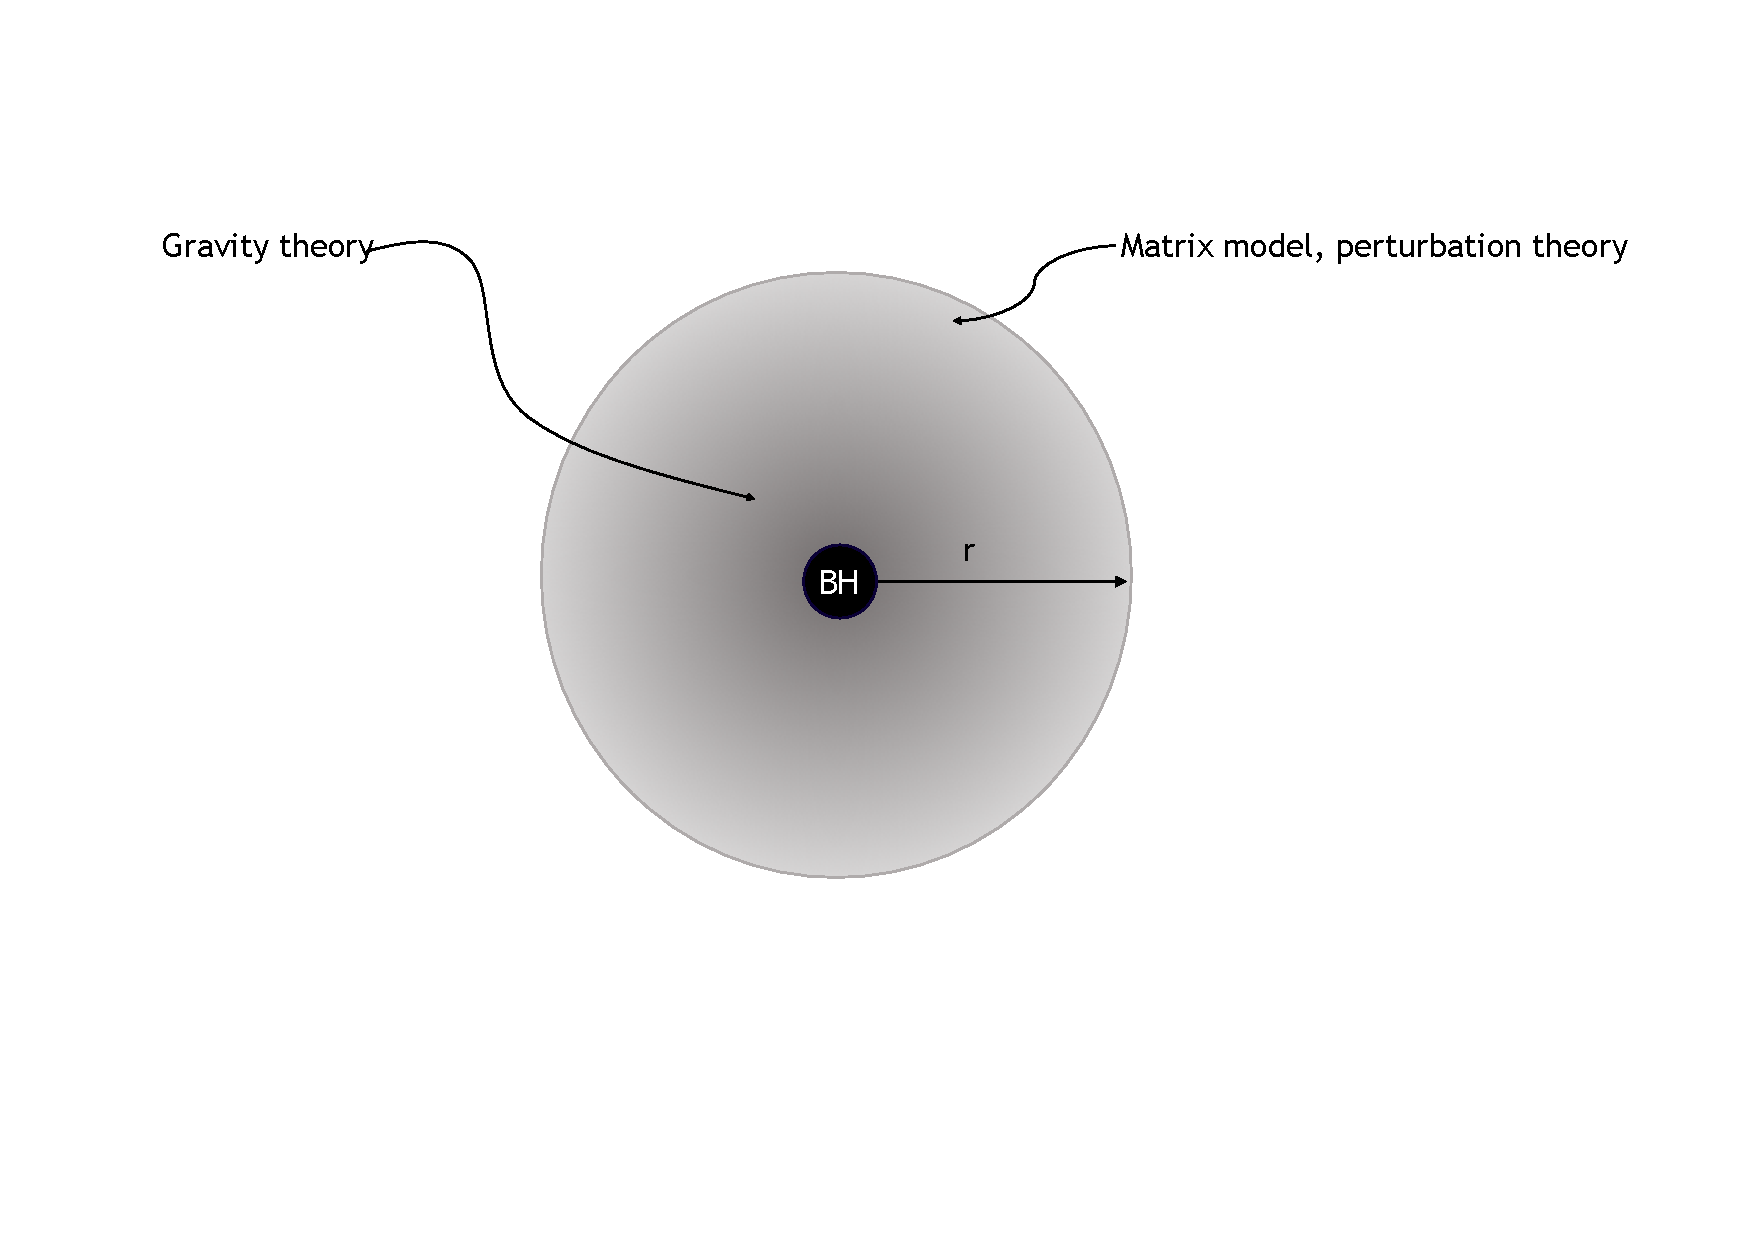
\includegraphics[scale=0.4]{bulk}
\caption{A pictorial representation of the regime of gravity and the regime of matrix model. In this way one can approximate different regimes with the help of the radial parameter $r$, the deformation parameter $\mu$ and the effective coupling $g=\frac{\lambda}{\mu^3}$.}
\label{bulk}
\end{figure}

\subsubsection{Force at zero temperature}
In this subsection we calculate the force that a D0-brane feels in the background of \eqref{trivialvac} which corresponds to the trivial vacuum in the matrix model side. We actually repeat the calculation of section \ref{classicalforce}. To this end we use \eqref{bosonicpart} with the data of \eqref{trivialvac}, fixing the spherical part of the metric. Doing this, in the non-relativistic limit, we get the action 
\be 
S_{D_0}\approx-T_0\int dt\left[e^{-\phi}H(r)^{-\frac{1}{4}}\left(1-\frac{1}{2}H(r)\left(\left(\frac{dz}{dt}\right)^2+\left(\frac{dr}{dt}\right)^2\right)\right)-A_1(r)\right]
\ee
From this DBI action, the potential could be read off as 
\be \label{potential}
V_{D_0}(r)=T_0\left[ e^{-\phi}H(r)^{-\frac{1}{4}}-A_1(r)\right].
\ee
We remind that \eqref{trivialvac} corresponds to a deformed version of the near horizon geometry of D0-branes. These D0-branes are in fact coincident and realize a $U(N)$ symmetry. When we treat one of them as a probe, then we actually break the symmetry to $U(N)\to U(N-1)\times U(1)$, giving a Higgs expectation value\footnote{We remind that we have set $\alpha'=1$, otherwise the Higgs expectation value would be $U=\frac{r}{\alpha'}$.}
 $r$. This corresponds to placing a single D0-brane at distance $r$ from the center.
 
We see the behavior of the force and the potential in figure \ref{F-V}. In fact we see an interesting behavior. Coming from large values of $r$ towards $r=0$ the D0-brane experiences different situations depending on $r$, i.e  the distance of the probe from the bunch. Where, by the term bunch we are referring to the constituents of the black hole-like solution \eqref{trivialvac} which in this case is a bunch of D0-branes. To make the point more clear, suppose that we fix $N$ to be very large $N>>1$ and vary $r$, keeping in mind the conditions \eqref{validsugra}. Indeed for large $r$, we see an attractive force which going towards the black hole-like core \footnote{Since we are at zero temperature, the horizon is located at $r=0$, so approaching the horizon means approaching the singularity here.} becomes repulsive . We give a more general comment on this in the next section \ref{transitionsection}, but there is a pattern behavior and can be described as follows: for sufficient large $N$ the probe will experience an attractive force far away from the core, but going towards the core will feel repulsive phenomena. We remind that the whole analysis is classical and is valid in the regime \eqref{validsugra}.  Nevertheless, at least \textit{qualitatively} this is in accordance with \cite{Hyakutake2014} where the same effect was observed in quantum corrected black 0-brane geometries and it was verified by simulations in \cite{Masanori2017}. Also, it deserves to be mentioned that  the steep curves of the potential and the force should not taken too seriously because they are outside the regime of validity \eqref{validsugra} of the classical supergravity geometry \eqref{trivialvac}. However, the behaviour seems to be independent of $N$ since the curves join going towards the core.
%\begin{figure}\label{smallN}
%	\centering
%\includegraphics[scale=0.5]{smallN}
%\end{figure}

What is interesting here  in contrast to the BFSS case, is the fact that repulsive phenomena can occur even classically and far away from the horizon if $N$ is sufficiently large. This is also the regime where the gravity description is valid, and we can understand this repulsive phenomenon as the R-R charge of the D0-branes. 

Physically, it is also interesting the fact that in this system if one tries to throw a D0-brane towards the bunch when $N$ is large, then it  should be thrown with enough energy such that it will be able to overcome the potential which is growing going towards the horizon and eventually merge with the bunch. One more observation is the fact that for different $N$ the minimum of the potential varies on $r$. In fact one can imagine that instead of just one D0-brane for probe we have many of them ($q\ll N$), then  these D0-branes could be in the minimum of the potential  on a specific distance $r$ or in a specific energy scale of the system, forming in this way a bound state with the bunch. 

It is known for the BMN model that there might be a tunneling effect between "nearby" vacua \cite{Lin2006a}, where the probability to tunnel is given by the exponential $e^{-\frac{N}{\lambda}}$ since it is mediated by instantons. $N$ is the number of the degrees of freedom (i.e D0-branes) and $\lambda$ the t'Hooft coupling. As a result in the regime we are interested in, the tunneling between different vacua is exponentially suppressed. 

\begin{figure}[h]
	\centering
	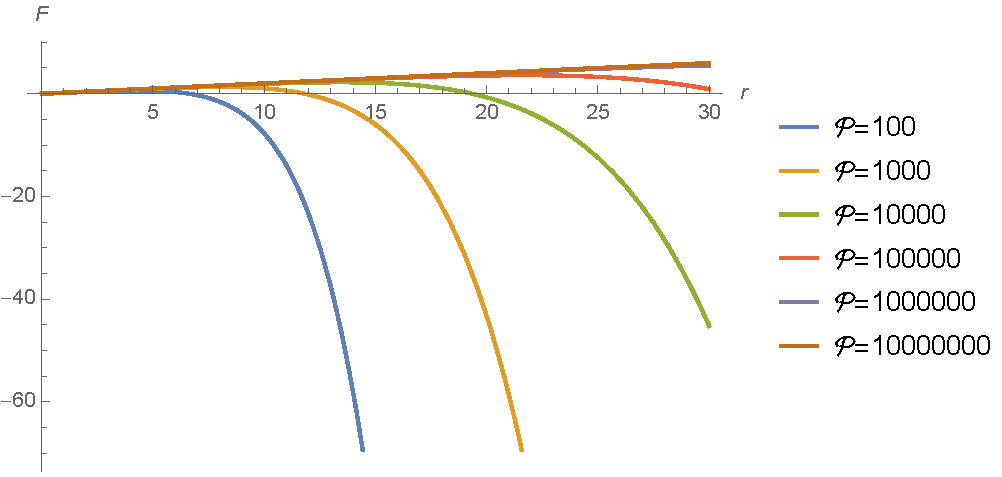
\includegraphics[scale=0.48]{force_tr_vac}
	\includegraphics[scale=0.48]{potential_tr_vac}
	\caption{The force (left) and potential (right) are plotted with respect to the radial coordinate $r$ for various values of $\mathcal{P}\sim N$.}
	\label{F-V}
\end{figure}

One might worry that since we are at zero temperature the force should be zero due to supersymmetry. However, we remind that so far we are analysing only the bosonic sector of the model and this is the force due to the bosonic degrees of freedom.  

\subsubsection{Force at finite temperature}\label{sectionfiniteT}
At finite temperature the BMN model has $\frac{1}{2}$- BPS states \cite{Berenstein2002}, \cite{Dasgupta2002} and we should expect the force to be present even if we consider fermions. Eventually, also we would like to make some contact with the quantum mechanics side. Note that this quantum mechanics however is a subsector of  the SYM theory. So
let us be a bit more illustrative here.  The parameters that control the vacua of the BMN, are the number\footnote{To be more precise it is the charge of the various D-branes.} of D2-branes $N_2$, the number of D5-branes $N_5$, and the number of D0-branes $N_0$, whose relation  is given as \cite{Lin2006}
\be 
N_2=\frac{N_0}{N_5}.
\ee 
Now, we remind that the trivial vacuum is dictated by $N_5=1, N_2=N_0=N$, with $N$ being the copies of the trivial ($j=0$) representation. This particular configuration is given in figure \ref{rzplane}. Then to understand the situation in the gauge theory side, we need to convert the gravity data to the gauge data. By direct comparison with \cite{Itzhaki1998}, we find the following \cite{Lin2006}\footnote{We supress $\mu$ dependence here by setting $\mu=1$ but we can restore it by dimensional analysis.}
\begin{align}
\rho_0^4=\frac{\pi^4}{2}g_{YM}^2 N~~,~~d=\frac{\pi}{2}N_5=\frac{\pi}{2}~~,~~\mathcal{Q}=\frac{\rho_0^4}{8}~~,~~  \mathcal{P}=2d\ \mathcal{Q}=\frac{\pi^5g_{YM}^2\ N}{16}.
\end{align}
Here, $\rho_0$ is the value of the coordinate $\rho$ on which the tip of the conducting disk lies (see figure \ref{rzplane}), $d$ is the charge of $N_5$ which is also the distance between the two conducting disks.  Before we continue, the above data reflect the repeated statement, that the size of the fivesphere is much larger than the one of $S^2$,  into the radius of the fivesphere  \cite{Lin2006}
\be 
\frac{R^2_{S^5}}{\alpha'}=4\pi\rho_0=4\pi\left(\frac{\lambda}{2}\right)^{\frac{1}{4}}.
\ee  


 We investigate the gravity solution at finite temperature $T$ in this vacuum. We can write the finite $T$ black brane solution as 
\begin{align}\label{finiteT} \nn
\frac{ds^2_T}{\alpha'}&=-H(r)^{-\frac{1}{2}}f(r)dt^2+16H(r)^{\frac{1}{2}}\left(dz^2+z^2d\Omega_2^2\right)+H(r)^{\frac{1}{2}}\left(\frac{dr^2}{f(r)}+r^2d\Omega_5^2\right),\\
\nn H(r)&=\frac{\lambda d_0}{r^7}~~,~~ e^\phi =2^6\left(\frac{\lambda 15\pi^5}{r^7}\right)^\frac{3}{4}~~,~~f(r)=1-\frac{r_0^7}{r^7},\\
\nn A_1(r)&=-\frac{r^7}{1920\pi^5\lambda}-\frac{7r^5}{960\pi^3\lambda}-\frac{7r^3}{192\pi \lambda}+\frac{r^2}{10}-\frac{7\pi r}{96\lambda}-\frac{3\pi^2}{5},\\
d_0&\equiv 240\pi^5~~,~~\lambda\equiv g^2_{YM}N~~,~~g_s=4\pi^2l_s^3\frac{\lambda}{N}~~,~~G_{10}=g_s^2l_s^8,
\end{align}
and the horizon is located at $r=r_0$, with $r_0$ representing the thermal energy scale.  This is useful to study thermodynamic properties of the system. Note that the horizon is dictated only from the radius of the five-sphere, reflecting the fact that this particular vacuum solution is due to a single fivebrane.  Indeed from this metric one can extract the temperature via the surface gravity 
\be 
T=\frac{7 r_0^{5/2}}{4\pi \sqrt{\lambda d_0}}
\ee 
but before we continue let us state when the gravity description is valid. In principle, the gravity solution due to the fivebrane is not well behaved and this is reflected from the fact that if $z$ is of order one, then the curvature of $S^2$ gives a different limit of validity. To fix this, we demand $z\gg 1$ \cite{Lin2006} such that the metric is well behaved. Thus, the curvature of the spheres is not too large from which we get the conditions 
\begin{align}
r&\lesssim \lambda^{1/3} ~~~~~~~\text{from the $S^5$},\\
r&\lesssim (\lambda z^4)^{1/7}~~\text{from the $S^2$},
\end{align}
where $z\sim\lambda^{\frac{1}{3}}$. In fact, we have shifted the problem to the size of the spheres, because sending $z\to \lambda^{1/3}$ means blowing up the twosphere. However, this is the "extremal" case when $z$ and $r$ are of the same order and the sizes of the spheres are equal, but in general we have  $z\ll r$. There is also one more constraint coming by demanding that the dilaton is not too large on the horizon which results in 
\be 
\lambda \beta^3\lesssim N^{10/7},
\ee
but for sufficiently large $N$ with respect to the combination $\lambda\beta^3$ the last condition is automatically satisfied.

\noindent 
The calculation of the force uses a variation of equation \eqref{potential},
\be \label{potentialfiniteT}
V_{D_0}(r)=T_0\left[ e^{-\phi}H(r)^{-\frac{1}{4}}f(r)^\frac{1}{2}-A_1(r)\right].
\ee 
 with the data of the finite temperature gravity solution \eqref{finiteT}. We expect qualitatively similar behavior as in the zero temperature system because the probe brane is a BPS state, and evaluating indeed we see the behavior in figure \ref{F-V-T}.
\begin{figure}[h]
	\centering 
	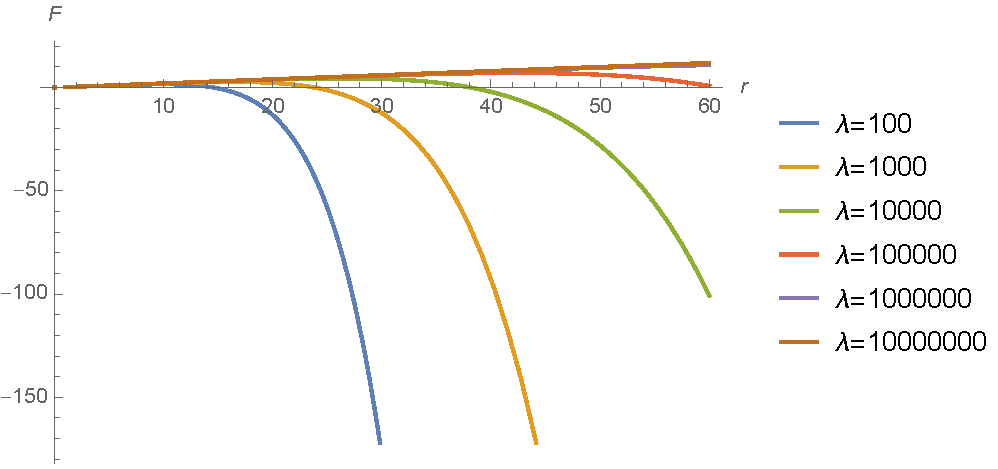
\includegraphics[scale=0.48]{FiniteTForce}
	\includegraphics[scale=0.48]{FiniteTpot}
	\caption{Finite temperature force (left) and potential (right) with respect to the radial coordinate $r$ (or equivalently temperature $T$). We observe a similar behavior as in figure \ref{F-V}. We have set for the horizon $r_0=1$ and $g_{YM}=1$. }
\label{F-V-T}
\end{figure}

\subsection{A note on phase transition}\label{transitionsection}
Here we discuss some aspects of Gregory-Laflamme instability \cite{Gregory93} regarding this model.
The parameter that controls most of the features here is  $N$. A useful interpretation is the number of D0-branes. Then this number controls the regimes of the theory, i.e the regimes where the gravity picture is valid or quantum corrections have to be taken into account. Then, we can imagine a situation where we start investigating a black hole, i.e for simplicity a Schwarzschild-like black hole,  when $N$ is large. In this limit, and for specific range of $r$ which is dictated by demanding the curvature not to be large, the supergravity description is valid. In addition, decreasing $N$ leads to a critical value $N\sim S$, where the number of D0-branes is the same order as the entropy of the system ($S$). This rather means that the constituents of the black hole (in this case the D0-branes) gives the entropy of the system. Intuitively, this makes sense since each D0-brane carries also a different degree of freedom, resulting in a different (micro)state and thus microstate counting gives the entropy.   We note that in the $N\gg S$ regime, we introduce a "needless" amount of degrees of freedom which due to supersymmetry they are in their ground state (energy of fermions cancel the one of bosons) . As one approaches the point $S\sim N$  from large $N$ in this specific value both the black hole and the black brane solutions have the same entropy. Further decreasing $N$ leads to a phase transition where the black hole transforms to a gas of D0-branes \cite{HorowitzCorr}, \cite{Horowitz1997}.  

The transition from a black hole description to a gas of D0-branes (or vice versa) can be motivated by some thermodynamic arguments as follows. Suppose that we have a system of gas D0-branes and a black hole with the same mass $M$. Then, we can estimate the entropies of the two systems as \cite{Horowitz1997}
\begin{align}
S_{\text{BH}}&\sim\left(l_{\text{pl}}/L^d\right)^{\frac{1}{D-3}}\sim \frac{M^{\frac{D-2}{D-3}}}{G_N^{D-3}}\\
S_{\text{gas}}&\sim N^{\frac{1	}{2}}\left(l_{\text{pl}}^9/L^d\right)^{\frac{1}{D-4}}\left(\frac{E_{LC}}{R}\right)^{\frac{D-2}{2(D-4)}}\sim N^{-\frac{1}{D-4}}\frac{M^{\frac{D-2}{D-4}}}{G_D^{D-4}}.
\end{align}
Let us fix the dimension of the spacetime to be $D=10$, which corresponds to $p=1$ compactified coordinate in $D=11-p$ expression. This gives 
\begin{align}
S_{\text{BH}}&\sim \frac{M^{\frac{8}{7}}}{G_{10}^7}\\
S_{\text{gas}}&\sim N^{-\frac{1}{6}}\frac{M^{\frac{8}{6}}}{G_{10}^{6}}.
\end{align}
From these expressions it is clear that for large $N$ the black hole has greater entropy than the D0 gas for a specific choice of mass. Thus in the large $N$ limit, the black hole is thermodynamically preferred, while for small values of $N$ the gas configuration is preferred. %On the other hand from \eqref{entropy} we see that the entropy in the trivial vacuum case is thermodynamically preferred for any value of $N$.

\noindent
A different way of thinking for this transition is the following. We remind that $N$ is also related with the boost in the compactified circle, in a sense that the larger the boost the larger the momentum and hence the larger the $N$. Then starting with small momenta in the eleven-dimensional circle, in the ten-dimensional picture this is a gas of D0-branes. As we boost more, $N$ increases until it reaches a value where the ten dimensional picture is that of a black hole.
\noindent
%When $N$ is large we can also explore the large $r$ region, i.e far away from the horizon.

 However, as we pointed out before the phenomenon we observe is (almost) universal in $N$\footnote{Small values of $N$ do not have the same behavior but in this case we should not really trust the gravity description.}, meaning that for every value of $N$ the system behaves the same. The D0-probe approaching from very far away tries to minimize its energy, and it is clear that this occurs on the minima of the potential. then approaching the horizon, it experiences a repulsive force. 



In our case, we can read off the temperature for which we have this instability. This can be understood from the above discussion and equation \eqref{entropy}. We want to find the "correspondence" point \cite{Horowitz1997}, \cite{HorowitzCorr}, by setting $S\sim N$. This leads to 
\be 
T_c=\frac{\lambda^{1/3}}{N^{5/3}},
\ee 
for the trivial vacuum. This temperature signals when the short of black hole \eqref{finiteT} has a Gregory-Laflamme instability \cite{Gregory93}.


\section{Synopsis}
\textcolor{red}{*Maybe extend the discussion a bit more*}

We have demonstrated gravitational behaviors of D-brane probes (D0-and D2-branes) for symmetry reduced pp-wave backgrounds. In particular for the D0-probe we have also studied its behavior for geometry which corresponds to the trivial vacuum of BMN. We have seen a repulsive behavior as we approach the "naked" singularity in the extremal case and the horizon in the non-extremal case. This most likely indicates that there is a mechanism that gives rise to repulsive forces as one approaches the singularity, but on the contrary one cannot really trust the supegravity description near the singularity since stringy physics should take the lead.

 However, the regime where we can trust supergravity depends on $N$ and hence for large $N$ one is already far away from the singularity.  In the same regime,  dynamically it seems more preferable that the D-brane probe will be at the minimum of the potential for specific $N$ forming in this way a bound state with the bunch. This follows from the analysis done in the main text and from the principle of least action.  From the same principle and figure \ref{F-V-T}, we conclude that if one perturbes the (D0-brane) probe energetically is more likely that it will head towards the bunch. This analysis holds only in the trivial vacuum geometry, and further studies need to be carried out to understand the situation of the non-trivial vacua which from geometric point of view are significantly more complicated.  The limit which we took to construct this geometry is also realized in simulations (\textcolor{red}{Cite to be appeared?}). We are referring to the large deformation of the geometry, as in the main text several times was emphasized  that the horizon of this geometry is of $S^5\times B^3$ topology with the size of $S^5$ being much bigger than that of $B^3$. However, one significant caveat of the construction is that we did not check explicitly that the vacuum geometries \eqref{trivialvac} and \eqref{finiteT} are solutions of Einstein's equations, but it is rather based on the spirit of \cite{Lin2006}.
 
\textcolor{red}{*Maybe remove*}
 It is tempting to think also about some short of enhanson mechanism \cite{Peet2000} in the following way.  In the $N$ D0-brane geometry the gauge symmetry is $U(N)$, then placing $q$ D0-probes with $q\ll N$ in a distance $r$ from the singularity created by the N D0-brane geometry, the symmetry breaks as $U(N)\to U(N-q)\times U(1)^q$. However it is not clear if such  a mechanism exists for the case of D0-branes.
 
  Understanding these bulk descriptions will be beneficial to extract meaningful physics when one also compares with the matrix model side both in analytic, and nowadays,  numerical results.      
  
 \subsection*{Acknowledgments}

  \appendix
  \section{Thermodynamics of the Vacuum}
  Here we calculate the entropy and the free energy of the trivial vacuum geometry. We can use the laws of black hole thermodynamics to evaluate the entropy, but for this one needs to know the geometry of the horizon. As it is known and can be easily seen from the metric \eqref{finiteT} we do not have a simple spherical geometry but we rather have $R\times B^3\times R \times S^5$. Thus, we have to find the area that this horizon spans such that we can use the Bekenstein-Hawking formula after switching to Einstein frame. Given an arbitrary metric that describes the horizon one can use the following formula
  \be \label{generalarea}
  \hat{A}=\int_\mathcal{H}\sqrt{\det{h}},
  \ee 
  where $\mathcal{H}$ is the geometry of the horizon, and $h$ is the induced metric on the horizon. Therefore, we can read this geometry off from \eqref{finiteT}, where it has a manifest $SO(3)\times SO(6)$ symmetry and the horizon has  $B^3\times S^5$  topology\footnote{We integrate also over $z$ with boundary values $z\in (0,\lambda^{1/3}]$, since at this case we form the maximal area for the horizon.}.  
  \noindent
  Furthermore, we can use the  Bekenstein-Hawking formula to evaluate the \textit{physical} entropy as
  \be 
  S=e^{-2\phi}\int_{B^3\times S^5}\sqrt{\det{h}}=\frac{64\pi^4 }{3}e^{-2\phi} \left(\frac{r}{l_s}\right)^5\left(\frac{z}{l_s}\right)^3H(r)^2=\frac{\frac{64\pi^4}{3}H(r_0)^{\frac{1}{2}}r_0^5z_0^3}{G_{10}},
  \ee 
  where in the last equality we have used $e^\phi=g_sH(r)^{3/4}$ for the dilaton, and $z\mapsto z_0$ which can be though either as the "extremal" energy scale due to $S^2$ that corresponds to $\frac{z_0}{\lambda^{1/3}}\sim\frac{\pi}{2}$, or as the distance between the infinite conducting plate and the first conducting plate in figure \ref{rzplane}.  
  
  Putting everything together we have 
  \be \label{entropy}
  S\approx N^2\left(\frac{T}{\lambda^{1/3}}\right)^{3/5},
  \ee  
  suppressing numbers in front of the right-hand side. 
  
  \noindent
  The free energy for the trivial vacuum follows from the first law of thermodynamics and gives 
  \be \label{freeE}
  \frac{F}{\lambda^{1/3}}\approx\frac{5}{8}N^2\left(\frac{T}{\lambda^{1/3}}\right)^{8/5}.
  \ee 
  
 
\nocite{*}
\bibliography{D0-BMN}
\bibliographystyle{utphysmendeley}




\end{document}